\documentclass[12pt]{article}
\usepackage{amsmath, amssymb}
\usepackage{geometry}
\usepackage{booktabs}
\usepackage{array}
\usepackage{enumitem}
\usepackage{titlesec}
\usepackage[dvipsnames, table]{xcolor}
\usepackage{fancyhdr}
\usepackage{tcolorbox}
\usepackage{microtype}
\usepackage{tikz}
\usetikzlibrary{shapes, arrows.meta, positioning}

\tcbuselibrary{skins, breakable}

\geometry{margin=1in, top=1in, bottom=1in}

% ── Colour palette ──────────────────────────────────────────
\definecolor{primary}{RGB}{74,  35,  90}   % deep royal purple
\definecolor{accent} {RGB}{22, 160, 133}   % muted teal
\definecolor{lightbg}{RGB}{245,238,248}    % light lavender
\definecolor{gold}   {RGB}{211, 84,   0}   % burnt orange
\definecolor{goldbg} {RGB}{254,245,232}    % warm cream
\definecolor{softgray}{RGB}{248,244,252}   % faint purple-grey
\definecolor{darktext}{RGB}{44,  62,  80}
\definecolor{green1}{RGB}{22, 160, 133}    % teal (= accent)
\definecolor{greenbg}{RGB}{232,247,243}    % light teal

% ── Page headers / footers ──────────────────────────────────
\pagestyle{fancy}
\fancyhf{}
\fancyhead[L]{\small\color{primary}\textbf{Statistical Inference}\;\textcolor{accent}{|}\;Mid Term Solutions}
\fancyhead[R]{\small\color{darktext}BS P-IV Mathematics}
\renewcommand{\headrulewidth}{0pt}
\fancyhead[C]{\color{accent}\rule[-1ex]{\textwidth}{1.2pt}}
\fancyfoot[C]{\small\color{darktext}\thepage}

% ── Section styling ─────────────────────────────────────────
\titleformat{\section}
  {\large\bfseries\color{primary}}
  {}
  {0em}
  {}
  [\color{accent}\rule{\linewidth}{2pt}]
\titlespacing*{\section}{0pt}{20pt}{10pt}

\titleformat{\subsection}
  {\normalsize\bfseries\color{accent}}
  {}
  {0em}
  {}

% ── tcolorbox styles ────────────────────────────────────────
\newtcolorbox{formulabox}{
  enhanced,
  colback=goldbg, colframe=gold, arc=5pt, boxrule=1.5pt,
  left=12pt, right=12pt, top=10pt, bottom=10pt,
  title={\small\bfseries Formula / Key Result},
  colbacktitle=gold!30, coltitle=darktext,
  attach boxed title to top left={xshift=12pt, yshift=-\tcboxedtitleheight/2},
  boxed title style={arc=3pt, colframe=gold, colback=gold!25, boxrule=1pt},
}

\newtcolorbox{problembox}{
  enhanced,
  colback=lightbg, colframe=primary, arc=5pt, boxrule=2pt,
  left=12pt, right=12pt, top=8pt, bottom=8pt,
  title={\small\bfseries Question},
  colbacktitle=primary, coltitle=white,
}

\newtcolorbox{conceptbox}{
  enhanced,
  borderline west={4pt}{0pt}{accent},
  colback=lightbg!55, colframe=white,
  arc=0pt, boxrule=0pt,
  left=12pt, right=8pt, top=6pt, bottom=6pt,
}

\newtcolorbox{answerbox}{
  enhanced,
  colback=greenbg, colframe=green1, arc=5pt, boxrule=1.5pt,
  left=12pt, right=12pt, top=8pt, bottom=8pt,
  title={\small\bfseries Answer},
  colbacktitle=green1!80, coltitle=white,
  attach boxed title to top left={xshift=12pt, yshift=-\tcboxedtitleheight/2},
  boxed title style={arc=3pt, colframe=green1, colback=green1!70, boxrule=1pt},
}

\newtcolorbox{observebox}{
  enhanced,
  colback=softgray, colframe=primary!50, arc=5pt, boxrule=1pt,
  left=12pt, right=12pt, top=8pt, bottom=8pt,
  title={\small\bfseries Key Points},
  colbacktitle=primary, coltitle=white,
}

\newcolumntype{C}[1]{>{\centering\arraybackslash}p{#1}}
\newcommand{\hcell}[1]{\textbf{\color{white}#1}}

\begin{document}

% ════════════════════════════════════════════════════════════
%  TITLE BANNER
% ════════════════════════════════════════════════════════════
\thispagestyle{empty}

\begin{tcolorbox}[
  enhanced, arc=0pt, boxrule=0pt,
  colback=primary, colframe=primary,
  left=16pt, right=16pt, top=18pt, bottom=14pt,
  borderline south={4pt}{0pt}{accent},
]
  \centering
  {\huge\bfseries\color{white} Statistical Inference}\\[6pt]
  {\large\color{lightbg} Mid Term Examination --- Step-by-Step Solutions}
\end{tcolorbox}

\vspace{4pt}

\begin{tcolorbox}[
  enhanced, arc=0pt, boxrule=0pt,
  colback=white, colframe=white,
  borderline north={1.5pt}{0pt}{accent!60},
  borderline south={1.5pt}{0pt}{accent!60},
  left=16pt, right=16pt, top=12pt, bottom=12pt,
]
  \begin{tabular}{p{3.2cm} p{9.5cm}}
    \textcolor{primary}{\textbf{Department:}}
      & \textbf{Department of Mathematics, SALU Khairpur} \\[4pt]
    \textcolor{primary}{\textbf{Class:}}
      & \textbf{BS P-IV} \quad|\quad First Semester \\[4pt]
    \textcolor{primary}{\textbf{Course:}}
      & \textbf{Statistical Inference} \\[4pt]
    \textcolor{primary}{\textbf{Date:}}
      & \textbf{25-03-2025} \quad|\quad Session: 2025 \\[4pt]
    \textcolor{primary}{\textbf{Prepared by:}}
      & \textbf{Nadir Ali Khan} \\
      & {\small\color{darktext}BS P-IV \quad|\quad First Semester 2025} \\
  \end{tabular}
\end{tcolorbox}

\vspace{14pt}

% ════════════════════════════════════════════════════════════
\section{Question \#1(a) --- Inferential Statistics}
% ════════════════════════════════════════════════════════════

\begin{problembox}
Explain Inferential Statistics and explain why and where inferential statistics are used. Give examples.
\end{problembox}

\subsection*{Definition}

\begin{conceptbox}
\textbf{Inferential Statistics} is the branch of statistics that uses data from a \emph{sample} to draw conclusions, make predictions, or test hypotheses about a larger \emph{population}. Unlike descriptive statistics (which merely summarise data), inferential statistics allows us to make inferences beyond the observed data.
\end{conceptbox}

\subsection*{Why Inferential Statistics?}

In practice it is impossible or impractical to collect data from every member of a population. Inferential statistics provides rigorous tools to:
\begin{enumerate}[noitemsep, topsep=6pt]
  \item \textbf{Estimate population parameters} (mean, proportion, variance) from sample statistics.
  \item \textbf{Test hypotheses} about population characteristics.
  \item \textbf{Quantify uncertainty} through confidence intervals and $p$-values.
  \item \textbf{Predict} future outcomes based on observed patterns.
\end{enumerate}

\subsection*{Where Inferential Statistics is Used}

\begin{center}
\begin{tabular}{p{3.5cm} p{9cm}}
\toprule
\rowcolor{primary}
\hcell{Field} & \hcell{Application} \\
\midrule
\rowcolor{lightbg!40}
Medicine & Clinical trials estimate drug effectiveness from a sample of patients. \\
Business & Market research uses sample surveys to predict consumer preferences. \\
\rowcolor{lightbg!40}
Quality Control & A manufacturer tests a sample of products to infer defect rates in the entire batch. \\
Social Sciences & Polling a sample of voters to forecast election results. \\
\rowcolor{lightbg!40}
Agriculture & Testing fertiliser on a few plots to draw conclusions about the whole farm. \\
\bottomrule
\end{tabular}
\end{center}

\subsection*{Examples}

\begin{formulabox}
\textbf{Example 1 (Estimation):}\\
A researcher measures the blood pressure of 200 patients (sample) and uses the sample mean $\bar{x} = 120\,\text{mmHg}$ to estimate the population mean $\mu$ with a 95\% confidence interval: $\mu \in (118,\; 122)$.\\[8pt]
\textbf{Example 2 (Hypothesis Testing):}\\
A company claims that its new drug reduces cholesterol by 15\%. A sample of 50 patients is tested and a $t$-test is used to either \emph{accept} or \emph{reject} this claim at the 5\% significance level.
\end{formulabox}

\newpage

% ════════════════════════════════════════════════════════════
\section{Question \#1(b) --- Mathematical Probability}
% ════════════════════════════════════════════════════════════

\begin{problembox}
Define the Concept of Mathematical Probability, mutually exclusive and non-mutually exclusive events, and shortly discuss the role of Probability in the field of Business studies.
\end{problembox}

\subsection*{Mathematical Probability}

\begin{conceptbox}
If a random experiment has $n$ equally likely outcomes and event $A$ can occur in $m$ of them, then the \textbf{probability of event $A$} is:
\[
  P(A) = \frac{m}{n} = \frac{\text{Number of favourable outcomes}}{\text{Total number of outcomes}}
\]
Probability always satisfies: $0 \le P(A) \le 1$, and $P(S) = 1$ where $S$ is the sample space.
\end{conceptbox}

\subsection*{Mutually Exclusive Events}

Two events $A$ and $B$ are \textbf{mutually exclusive} (disjoint) if they cannot occur simultaneously:
\[
  A \cap B = \emptyset \quad \Longrightarrow \quad P(A \cup B) = P(A) + P(B)
\]
\textit{Example:} Rolling a die --- the events ``getting a 2'' and ``getting a 5'' are mutually exclusive.

\subsection*{Non-Mutually Exclusive Events}

Two events $A$ and $B$ are \textbf{non-mutually exclusive} if they can occur together. We use the \textbf{General Addition Rule}:
\[
  P(A \cup B) = P(A) + P(B) - P(A \cap B)
\]
\textit{Example:} Drawing a card --- the events ``getting a red card'' and ``getting a king'' can both happen (red king), so they are non-mutually exclusive.

\subsection*{Role of Probability in Business Studies}

\begin{observebox}
\begin{itemize}[noitemsep]
  \item \textbf{Risk Assessment:} Businesses use probability to assess financial risk and uncertainty in investments.
  \item \textbf{Decision Making:} Expected value calculations help managers choose optimal strategies under uncertainty.
  \item \textbf{Quality Control:} Probability models determine acceptable defect rates in production.
  \item \textbf{Insurance \& Finance:} Actuaries compute premiums based on the probability of claims.
  \item \textbf{Market Research:} Survey data is used to estimate the probability that consumers prefer a product.
\end{itemize}
\end{observebox}

\newpage

% ════════════════════════════════════════════════════════════
\section{Question \#2(a) --- Vehicle Assembly Probabilities}
% ════════════════════════════════════════════════════════════

\begin{problembox}
A vehicle builder assembles cars and bikes at four locations (A, B, C and D) according to the accompanying table. Find:\\
(i) P(a vehicle selected at random is a bike OR was assembled at location C)\\
(ii) P(a vehicle selected at random is a car OR was assembled at location B)\\
(iii) P(a vehicle selected at random is a bike AND was assembled at location A)
\end{problembox}

\subsection*{Data Table and Totals}

\begin{center}
\begin{tabular}{C{2.8cm} C{1.5cm} C{1.5cm} C{1.5cm} C{1.5cm} C{1.8cm}}
\toprule
\rowcolor{primary}
\hcell{Vehicle Type} & \hcell{A} & \hcell{B} & \hcell{C} & \hcell{D} & \hcell{Total} \\
\midrule
\rowcolor{lightbg!40}
Car & 10 & 7 & 9 & 5 & \textbf{31} \\
Bike & 16 & 9 & 4 & 10 & \textbf{39} \\
\midrule
\rowcolor{primary}
\hcell{Total} & \hcell{26} & \hcell{16} & \hcell{13} & \hcell{15} & \hcell{70} \\
\bottomrule
\end{tabular}
\end{center}

\vspace{8pt}
\noindent\textbf{Grand Total} $= 70$ vehicles.

\subsection*{Part (i) --- P(Bike OR Location C)}

Using the General Addition Rule:
\[
  P(\text{Bike} \cup \text{C}) = P(\text{Bike}) + P(\text{C}) - P(\text{Bike} \cap \text{C})
\]
\[
  = \frac{39}{70} + \frac{13}{70} - \frac{4}{70}
  = \frac{48}{70}
\]

\begin{answerbox}
\[
  P(\text{Bike OR Location C}) = \frac{48}{70} = \frac{24}{35} \approx \mathbf{0.686}
\]
\end{answerbox}

\subsection*{Part (ii) --- P(Car OR Location B)}

\[
  P(\text{Car} \cup \text{B}) = P(\text{Car}) + P(\text{B}) - P(\text{Car} \cap \text{B})
\]
\[
  = \frac{31}{70} + \frac{16}{70} - \frac{7}{70}
  = \frac{40}{70}
\]

\begin{answerbox}
\[
  P(\text{Car OR Location B}) = \frac{40}{70} = \frac{4}{7} \approx \mathbf{0.571}
\]
\end{answerbox}

\subsection*{Part (iii) --- P(Bike AND Location A)}

This is a direct joint probability (intersection):
\[
  P(\text{Bike} \cap \text{A}) = \frac{16}{70}
\]

\begin{answerbox}
\[
  P(\text{Bike AND Location A}) = \frac{16}{70} = \frac{8}{35} \approx \mathbf{0.229}
\]
\end{answerbox}

\newpage

% ════════════════════════════════════════════════════════════
\section{Question \#2(b) --- College Enrollment Survey}
% ════════════════════════════════════════════════════════════

\begin{problembox}
A college has an undergraduate enrollment of 3000. Of these, 860 are Business Majors (Event A) and 1400 are women (Event B). 375 of the business majors are women. The college newspaper staff is conducting a poll and selects undergraduate students at random.\\
(i)   What is the probability that a student selected is a woman \textbf{and} a business major?\\
(ii)  What is the probability that a student selected is a woman \textbf{and not} a business major?\\
(iii) Draw a Venn Diagram.
\end{problembox}

\subsection*{Given Information}

\[
  n(S) = 3000, \quad n(A) = 860, \quad n(B) = 1400, \quad n(A \cap B) = 375
\]
\[
  P(A) = \frac{860}{3000}, \quad P(B) = \frac{1400}{3000}, \quad P(A \cap B) = \frac{375}{3000}
\]

\subsection*{Part (i) --- P(Woman AND Business Major)}

\[
  P(B \cap A) = \frac{375}{3000} = \frac{1}{8}
\]

\begin{answerbox}
\[
  P(\text{Woman AND Business Major}) = \frac{375}{3000} = \frac{1}{8} = \mathbf{0.125}
\]
\end{answerbox}

\subsection*{Part (ii) --- P(Woman AND NOT Business Major)}

\[
  P(B \cap A') = P(B) - P(B \cap A) = \frac{1400}{3000} - \frac{375}{3000} = \frac{1025}{3000}
\]

\begin{answerbox}
\[
  P(\text{Woman AND NOT Business Major}) = \frac{1025}{3000} = \frac{41}{120} \approx \mathbf{0.342}
\]
\end{answerbox}

\subsection*{Part (iii) --- Venn Diagram}

\begin{center}
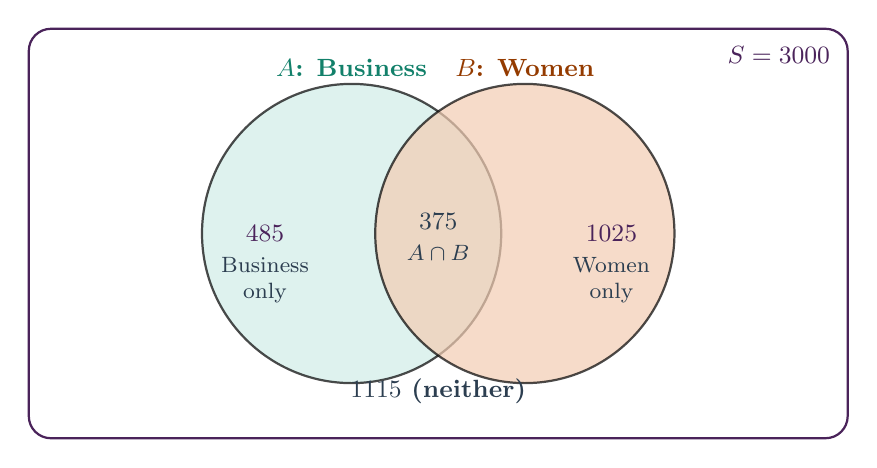
\begin{tikzpicture}
  % Bounding rectangle (sample space)
  \draw[thick, primary, rounded corners=8pt]
    (-5.2,-2.6) rectangle (5.2,2.6);
  \node[anchor=north east, color=primary, font=\small\bfseries] at (5.1,2.5) {$S = 3000$};

  % Circle A (Business Majors)
  \draw[thick, fill=accent!20, opacity=0.7] (-1.1,0) circle (1.9cm);
  % Circle B (Women)
  \draw[thick, fill=gold!30, opacity=0.7] ( 1.1,0) circle (1.9cm);

  % Labels inside regions
  % Only in A (Business but not Women)
  \node[font=\small\bfseries, color=primary] at (-2.2,0) {$485$};
  \node[font=\footnotesize, color=darktext] at (-2.2,-0.4) {Business};
  \node[font=\footnotesize, color=darktext] at (-2.2,-0.75) {only};

  % Intersection
  \node[font=\small\bfseries, color=darktext] at (0,0.15) {$375$};
  \node[font=\footnotesize, color=darktext] at (0,-0.25) {$A \cap B$};

  % Only in B (Women but not Business)
  \node[font=\small\bfseries, color=primary] at (2.2,0) {$1025$};
  \node[font=\footnotesize, color=darktext] at (2.2,-0.4) {Women};
  \node[font=\footnotesize, color=darktext] at (2.2,-0.75) {only};

  % Outside both circles
  \node[font=\small\bfseries, color=darktext] at (0,-2.0) {$1115$ (neither)};

  % Circle labels
  \node[font=\bfseries\small, color=accent!80!black] at (-1.1, 2.1) {$A$: Business};
  \node[font=\bfseries\small, color=gold!70!black] at ( 1.1, 2.1) {$B$: Women};
\end{tikzpicture}
\end{center}

\begin{observebox}
\textbf{Verification of cell counts:}\\[4pt]
$\bullet$\ Business only: $860 - 375 = 485$ \quad
$\bullet$\ Women only: $1400 - 375 = 1025$ \quad
$\bullet$\ Both: $375$\\
$\bullet$\ Neither: $3000 - 485 - 375 - 1025 = 1115$\\
$\bullet$\ Total: $485 + 375 + 1025 + 1115 = 3000$ \quad $\checkmark$
\end{observebox}

\newpage

% ════════════════════════════════════════════════════════════
\section{Question \#3(a) --- Cars Drawn Without Replacement}
% ════════════════════════════════════════════════════════════

\begin{problembox}
Consider an experiment in which two cars are drawn from a company containing one Alto car, two Swift cars, and three Suzuki Carry (the first one is not replaced before the second is drawn). Find the indicated probabilities:\\
(i)   Selecting two Suzuki Carry cars\\
(ii)  Drawing two Swift cars\\
(iii) Drawing two cars of different types
\end{problembox}

\subsection*{Setup}

\[
  \text{Alto (A)} = 1, \quad \text{Swift (S)} = 2, \quad \text{Suzuki Carry (C)} = 3, \quad \text{Total} = 6
\]

Total ways to choose 2 cars from 6 \textbf{without replacement}:
\[
  \binom{6}{2} = \frac{6!}{2!\,4!} = \mathbf{15}
\]

\subsection*{Part (i) --- P(Two Suzuki Carry)}

Favourable outcomes: choose 2 from 3 Suzuki Carry cars:
\[
  \binom{3}{2} = 3
\]

\begin{answerbox}
\[
  P(\text{2 Suzuki Carry}) = \frac{\dbinom{3}{2}}{\dbinom{6}{2}} = \frac{3}{15} = \frac{1}{5} = \mathbf{0.2}
\]
\end{answerbox}

\subsection*{Part (ii) --- P(Two Swift)}

Favourable outcomes: choose 2 from 2 Swift cars:
\[
  \binom{2}{2} = 1
\]

\begin{answerbox}
\[
  P(\text{2 Swift}) = \frac{\dbinom{2}{2}}{\dbinom{6}{2}} = \frac{1}{15} \approx \mathbf{0.067}
\]
\end{answerbox}

\subsection*{Part (iii) --- P(Two Different Types)}

\textbf{Method: Complement.} First find P(same type):

\[
  P(\text{same type}) = \frac{\dbinom{3}{2} + \dbinom{2}{2} + \dbinom{1}{2}}{15}
  = \frac{3 + 1 + 0}{15} = \frac{4}{15}
\]

Note: $\dbinom{1}{2} = 0$ since you cannot choose 2 from 1 Alto car.

\[
  P(\text{different types}) = 1 - P(\text{same type}) = 1 - \frac{4}{15} = \frac{11}{15}
\]

\textbf{Verification by direct count:} Pairs of different types $=$ (Alto,Swift) + (Alto,Carry) + (Swift,Carry)
$= 1\!\times\!2 + 1\!\times\!3 + 2\!\times\!3 = 2+3+6 = 11$ \quad $\checkmark$

\begin{answerbox}
\[
  P(\text{Different Types}) = \frac{11}{15} \approx \mathbf{0.733}
\]
\end{answerbox}

\newpage

% ════════════════════════════════════════════════════════════
\section{Question \#3(b) --- Playing Card Probabilities}
% ════════════════════════════════════════════════════════════

\begin{problembox}
Consider an experiment in which one card is randomly selected from a standard deck of 52 playing cards. Find the indicated probabilities:\\
(i)   Neither a face card nor a club\\
(ii)  A red colour card or not a king\\
(iii) An ace and a diamond
\end{problembox}

\subsection*{Standard Deck Reference}

{\small
\begin{center}
\begin{tabular}{lccccr}
\toprule
\rowcolor{primary}
\hcell{Category} & \hcell{Hearts} & \hcell{Diamonds} & \hcell{Clubs} & \hcell{Spades} & \hcell{Total} \\
\midrule
\rowcolor{lightbg!40}
Face cards (J, Q, K) & 3 & 3 & 3 & 3 & 12 \\
Aces & 1 & 1 & 1 & 1 & 4 \\
\rowcolor{lightbg!40}
Number cards (2--10) & 9 & 9 & 9 & 9 & 36 \\
\midrule
\rowcolor{primary}
\hcell{Total} & \hcell{13} & \hcell{13} & \hcell{13} & \hcell{13} & \hcell{52} \\
\bottomrule
\end{tabular}
\end{center}
}

\vspace{8pt}
Red cards = Hearts $\cup$ Diamonds $= 26$. \quad
Kings = 4. \quad Red kings = 2.

\subsection*{Part (i) --- P(Neither Face Card nor Club)}

Let $F$ = face card, $C$ = club.
\[
  n(F) = 12, \quad n(C) = 13, \quad n(F \cap C) = 3 \;\;(\text{J}\clubsuit,\text{Q}\clubsuit,\text{K}\clubsuit)
\]
\[
  n(F \cup C) = 12 + 13 - 3 = 22
\]
\[
  n(\overline{F \cup C}) = 52 - 22 = 30
\]

\begin{answerbox}
\[
  P(\text{neither face card nor club}) = \frac{30}{52} = \frac{15}{26} \approx \mathbf{0.577}
\]
\end{answerbox}

\subsection*{Part (ii) --- P(Red Card OR Not a King)}

Let $R$ = red card, $K'$ = not a king.
\[
  n(R) = 26, \quad n(K') = 48, \quad n(R \cap K') = 26 - 2 = 24 \;\;(\text{red non-kings})
\]

Using the Addition Rule:
\[
  P(R \cup K') = P(R) + P(K') - P(R \cap K') = \frac{26}{52} + \frac{48}{52} - \frac{24}{52} = \frac{50}{52}
\]

\textit{Alternative:} The only cards \emph{not} in $R \cup K'$ are black kings ($\spadesuit K, \clubsuit K$) $= 2$ cards.
$\Rightarrow P = (52-2)/52 = 50/52$ \quad $\checkmark$

\begin{answerbox}
\[
  P(\text{Red card OR Not a King}) = \frac{50}{52} = \frac{25}{26} \approx \mathbf{0.962}
\]
\end{answerbox}

\subsection*{Part (iii) --- P(Ace AND Diamond)}

This asks for the probability of drawing the \textbf{Ace of Diamonds} --- a single specific card:
\[
  n(\text{Ace} \cap \text{Diamond}) = 1
\]

\begin{answerbox}
\[
  P(\text{Ace AND Diamond}) = \frac{1}{52} \approx \mathbf{0.019}
\]
\end{answerbox}

\vspace{20pt}

\begin{formulabox}
\textbf{Summary of All Results}\\[8pt]
\begin{tabular}{p{1.3cm} p{1.3cm} p{8.5cm} p{2.5cm}}
\hline
\textbf{Q} & \textbf{Part} & \textbf{Event} & \textbf{Probability} \\
\hline
2(a) & (i) & Bike OR Location C & $\dfrac{24}{35} \approx 0.686$ \\[6pt]
2(a) & (ii) & Car OR Location B & $\dfrac{4}{7} \approx 0.571$ \\[6pt]
2(a) & (iii) & Bike AND Location A & $\dfrac{8}{35} \approx 0.229$ \\[6pt]
2(b) & (i) & Woman AND Business Major & $\dfrac{1}{8} = 0.125$ \\[6pt]
2(b) & (ii) & Woman AND NOT Business & $\dfrac{41}{120} \approx 0.342$ \\[6pt]
3(a) & (i) & Two Suzuki Carry & $\dfrac{1}{5} = 0.2$ \\[6pt]
3(a) & (ii) & Two Swift & $\dfrac{1}{15} \approx 0.067$ \\[6pt]
3(a) & (iii) & Different Types & $\dfrac{11}{15} \approx 0.733$ \\[6pt]
3(b) & (i) & Neither Face nor Club & $\dfrac{15}{26} \approx 0.577$ \\[6pt]
3(b) & (ii) & Red OR Not King & $\dfrac{25}{26} \approx 0.962$ \\[6pt]
3(b) & (iii) & Ace AND Diamond & $\dfrac{1}{52} \approx 0.019$ \\
\hline
\end{tabular}
\end{formulabox}

\end{document}
